\documentclass[11pt,letterpaper]{report}
\usepackage{amssymb,amsfonts,color,graphicx,amsmath,enumerate}
\usepackage{amsthm}

\newcommand{\naturals}{\mathbb{N}}
\newcommand{\integers}{\mathbb{Z}}
\newcommand{\complex}{\mathbb{C}}
\newcommand{\reals}{\mathbb{R}}
\newcommand{\mcal}[1]{\mathcal{#1}}
\newcommand{\rationals}{\mathbb{Q}}
\newcommand{\field}{\mathbb{F}}
\newcommand{\Var}{\text{Var}}
\newcommand{\ind}{\mathbbm{1}}
\newcommand{\Cov}{\text{Cov}}

\newenvironment{solution}
{\begin{proof}[Solution]}
{\end{proof}}

\voffset=-3cm
\hoffset=-2.25cm
\textheight=24cm
\textwidth=17.25cm
\addtolength{\jot}{8pt}
\linespread{1.3}

\begin{document}
\begin{center}
{\bf \Large Math 180B - Primitive Roots and Indices}
\vspace{0.2cm}
\hrule
\end{center}

\begin{enumerate}
	\item Suppose $\integers/n\integers$ has a primitive root ($n$ not necessarily prime). How many primitive roots does it have?

	\vfill

	\item You are given the table of powers base 2, modulo 37.\\
	\centerline{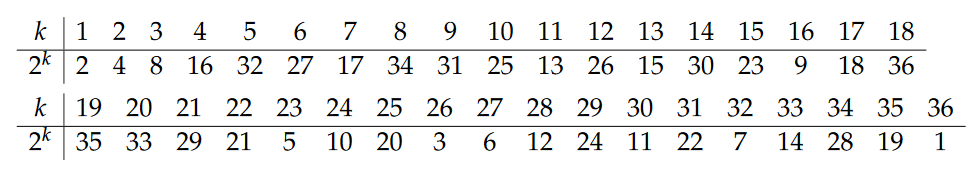
\includegraphics[scale=0.6]{table.PNG}}
	Use the table to find all solutions to the following congruences.
	\begin{enumerate}[(a)]
		\item $12x\equiv 23$
		\item $5x^{23}\equiv 18$
		\item $x^{12} \equiv 11$
		\item $7x^{20}\equiv 34$
	\end{enumerate}

	\vfill

	\item If $r$ and $r'$ are both primitive roots of the odd prime $p$, show that for $(a, p)= 1$,
	\[
	ind_{r'}\ a = (ind_r\ a)(ind_{r'}\ r)\pmod{p-1}.
	\]
	What other formula does this remind you of?

	\vfill

	\item Given the congruence $x^3\equiv a\pmod{p}$, where $p\geq 5$ is a prime and $(a, p) = 1$, prove the following:
	\begin{enumerate}[(a)]
		\item If $p\equiv 1\pmod{6}$, then the congruence has either no solutions or three incongruent solutions modulo $p$.
		\vfill
		\item If $p\equiv 5\pmod{6}$, then the congruence has a unique solution modulo $p$.
	\end{enumerate}

	\vfill

	\item 

	\vfill Suppose that $g$ is a primitive root modulo $p$, where $p$ is an odd prime.
	\begin{enumerate}[(a)]
		\item Let $n$ be the order of $g$ modulo $p^2$. Prove that $p-1\mid n$.
		\vfill
		\item Since $g$ is a primitive root modulo $p$, we have $g^{p-1}=1+up$ for some $u\in \integers$. Suppose that $p\nmid u$. Use the binomial theorem to prove that
		\[
		g^{t(p-1)}\equiv 1\mod{p^2}\iff p\mid t
		\]

		\vfill

		\item Explain why $g$ is a primitive root modulo $p^2$.
		\vfill
	\end{enumerate}
\end{enumerate}

\end{document}